\documentclass[a4paper, 12pt]{report}

% Adapté du tempate TER-M1 de l'Université de Paris

%%%%%%%%%%%%
% Packages %
%%%%%%%%%%%%

\usepackage[french]{babel}
%\usepackage{hyperref}
\usepackage[noheader]{packages/sleek}
\usepackage{packages/sleek-title}
\usepackage[french]{packages/sleek-theorems}
\usepackage{packages/sleek-listings}
\usepackage{tikz}
\usepackage[french,lined]{algorithm2e}	
\usepackage{pdfpages}
\usepackage{graphicx}
\graphicspath{ {./images/} }

\SetKwInput{KwResult}{R\'esultat}
\SetKw{KwInput}{Entr\'ees}
%%%%%%%%%%%%%%
% Title-page %
%%%%%%%%%%%%%%

\logo{./resources/img/logo_science.png}
\institute{Sorbonne Université}
\faculty{Master ANDROIDE}
\title{Apprentissage social et imitation pour la robotique en essaim}
\subtitle{UE de projet M1}
\author{Alessia \textsc{Loi} -- Dorian \textsc{LANCELIN}}
\date{2022}



%%%%%%%%%%%%%%%%https://www.overleaf.com/project/6012bd305aee4065605e8f1d
% Bibliography %
%%%%%%%%%%%%%%%%

\addbibresource{./resources/bib/references.bib}

%%%%%%%%%%
% Others %
%%%%%%%%%%

\lstdefinestyle{latex}{
    language=TeX,
    style=default,
    %%%%%
    commentstyle=\ForestGreen,
    keywordstyle=\TrueBlue,
    stringstyle=\VeronicaPurple,
    emphstyle=\TrueBlue,
    %%%%%
    emph={LaTeX, usepackage, textit, textbf, textsc}
}

\FrameTBStyle{latex}

\def\tbs{\textbackslash}

%%%%%%%%%%%%
% Document %
%%%%%%%%%%%%

\begin{document}
    \maketitle
    \romantableofcontents

    \chapter{Introduction}
	L'objectif de ce projet est de trouver des outils permettant à des robots avec une mémoire très limitée d'apprendre à réaliser une tâche par l'observation des mouvements d'autres robots ayant les mêmes spécifications.
Dans cette optique, on considèrera que les robots ont des moyens de communication limités voire inexistants si possible.
En utilisant des agents au comportement prédéfini, nommés ici les experts, capables de réaliser au mieux la tâche envisagée et des robots apprenants, on pourra toujours observer une convergeance vers le comportement de l'expert dans les cas où l'apprentissage se fait uniquement dans le sens expert-apprenant.
    Dans certains cas particuliers, des méthodes explorées permettent à l'apprentissage apprenant-apprenant d'accélerer cette convergeance. 
    
    Ce projet a été encadré par messieurs Nicolas Bredeche et Stéphane Doncieux.  
    
    L'ensemble des codes utilisés afin d'obtenir les résultats décrits dans le document suivant sont disponibles sur notre dépôt \href{https://github.com/aerrynn/M1_Projet_ASIRE}{github}. 

    \chapter{État de l'art}
    Aujourd'hui, la plupart des algorithmes d'apprentissage utilisés en robotique en essaim sont soit déterministes, soit axés sur l'apprentissage par transfert de poids de neurones, à l'instar de l'algorithme HIT-EE\footnote{Nicolas Bredeche and Nicolas Fontbonne. 2022. Social learning in swarm robotics. Philos. Trans. R. Soc. B Biol. Sci. 377, 1843 (January 2022), 20200309. DOI:https://doi.org/10.1098/rstb.2020.0309} qui nous a servi de base pour le projet.
    
    HIT-EE est un algorithme d'apprentissage en ligne qui suit un principe simple : Chaque agent subit une phase d'évaluation durant laquelle il ne peut transmettre son patrimoine mais reçoit les messages d'autres agents. A l'issue de cette phase, pour chaque message reçu, Si sa fitness est inférieure à celle de l'émetteur, il copie une partie des poids de l'émetteur. Une fois tous les messages lus, son patrimoine peut muter avec une probabilité donnée. Enfin si son patrimoine a changé durant au moins l'une des deux phases précedentes, il recommence sa phase d'évaluation.
    
    \chapter{Contribution}
   
    \section{Choix de l'expérimentation : La tâche de fourragement}
    Dans le but d'évaluer la capacité d'apprentissage par comportement de notre essaim de robots, on a reproduit l'expérience de fourragement et l'avons simulée à l'aide de Roborobo.
    L'évaluation en elle-même se fait sur la quantité d'objets capturés par un agent sur une fenêtre de temps donnée (sliding window). On considèrera qu'il n'y a pas de perte d'informations lors du transfert, c'est-à-dire que l'apprenant est capable de voir tout ce que voit l'expert.
    
    On définit ainsi les paramètres de l'expérience :
    \begin{itemize}
    \item Taille de la population : 100 agents
    \item Nombre d'experts : 10
    \item Nombre d'apprenants : 90
    \item Nombre d'objets : 100
    \item Taille de l'arène : 1400x800 px
    \item Taille des robots : 5x5 px
    \item Nombre de senseurs : 16 ou 24
    \item Distance des senseurs : 16 ou 24 (8 senseurs, capable de distinguer le type de l'objet et la distance à ce dernier)
    \item Durée d'une expérience : 20,000 steps
    \item Nombre de répétions de l'expérience : 5
    \end{itemize}

Les différents experts suivent un comportement donné.
L'un sous forme de génome, c'est-à-dire 100 couple observations-actions.
Et le second dont l'objectif est d'éviter les obstacles (qu'ils soient des murs ou d'autres robots) tout en se focalisant sur le ramassage des objets dès que possible, obtenu par simple succession de conditions.


	\section{Méthode par transmission de comportements}
	On considère que chaque individu possède une base de données de traces comportamentales, utile à stocker les comportements qu'un individu expert lui a envoyé lorsque les deux robots se sont croisés.
	
	La base de données de chaque individu expert est initialisée au début de l'expérience : elle contient 100 traces pré-définies et n'évolue pas au cours du temps. Parmi toutes les traces possibles, les 100 traces que nous avons sélectionnées permettent aux individus experts d'être efficaces dans le contournement d'obstacles que ce soit des murs ou des robots pour prévenir les blocages et la collecte d'objets lorsqu'un objet se trouve dans le périmètre perceptible des senseurs.
	
	Une trace comportementale est un couple $( s_t, a_t )^T$, avec :
	\begin{itemize}
	\item $s_t$ : l'état courant du contexte, qui correspond à une liste de 24 valeurs des senseurs étendus. L'état courant est de la forme 
    $(s_1, s_2, s_3, ..., s_n)$ avec $n$ le nombre de senseurs du robot. 
	\item $a_t$ : l'action à appliquer en fonction du contexte sensoriel rélévé. L'action associée est de la forme $[t,r]$ avec $t$ le degré de transition et $r$ le dégré de rotation.
	\item $T$ : le temps de croisement des deux trajectoires, exprimé en nombre de steps. 
	\end{itemize}


	La base de données de chaque individu focal évolue au cours du temps. Au départ, elle contient une seule trace correspondant à un comportement par défaut à appliquer lorsqu'aucun des senseurs ne perçoit d'élement de l'environnement. Chaque fois que les trajectoires d'un individu focal et d'un individu expert se croisent, l'expert envoie une partie de ses traces à l'apprenant, qui enrichit ainsi sa collection de traces.
	
    L'ensemble de traces comportementales d'un individu focal constitue la base d'exemples (senseurs) et étiquettes (actions) qui sera utilisée pour l'entraînement et la prédiction des algorithmes d'apprentissage.
    
    \:
    
    \textbf{Protocole expérimental spécifique à cette partie:} 
    
    A chaque début d'évaluation, les conditions initiales sont réinitialisées, notamment:
    \begin{itemize}
	\item la position de tous les individus
    \item la base de données de comportements
    \item la performance de chaque individu (exprimée en nombre d'objets collectés)
	\end{itemize}
    
    
    Remarque : Pour l'algorithme de rétropropagation du gradient, les poids du réseau de neurones ne seront pas réinitialisés d'une évaluation à l'autre, dans le but de raffiner les poids précédemment obtenus en les testant dans un nouveau contexte.
    
    Les graphiques de distance sont obtenus ainsi:
    \begin{itemize}
        \item A chaque step, nous capturons l'univers aperçu par un individu expert, en enregistrant l'état qu'il détecte (liste de 24 senseurs) et l'action correspondante effectuée.
        \item A $t = 1000$ steps, nous comparons les individus focaux en faisant la somme de la distance euclidienne entre leur choix d'action pour chaque observation de l'expert, et l'action effectuée par l'expert pour l'ensemble des données enregistrées.
        \item Nous répétons la même technique à $t = 2500$ steps et à $t = 6000$ steps, ensuite nous comparons les résutats sur la tranche de $t = 0$ steps à $t = 2500$ steps.
    \end{itemize}


	
	
    \subsection{Apprentissage par rétropropagation du gradient}
    L'apprentissage par rétropropagation du gradient permet d'observer une évolution fluide du comportement des individus focaux : les trajectoires dessinent des ellipses qui deviennent progressivement plus larges et ouvertes au cours du temps. En présence d'obstacles, les individus répondent rapidement pour le contournement des murs et nous observons qu'il ne se crée pas d'interblocage avec les autres robots. De manière moins importante par rapport aux experts, nous remarquons aussi la reconnaissance d'objets.
    //REVOIR
    
    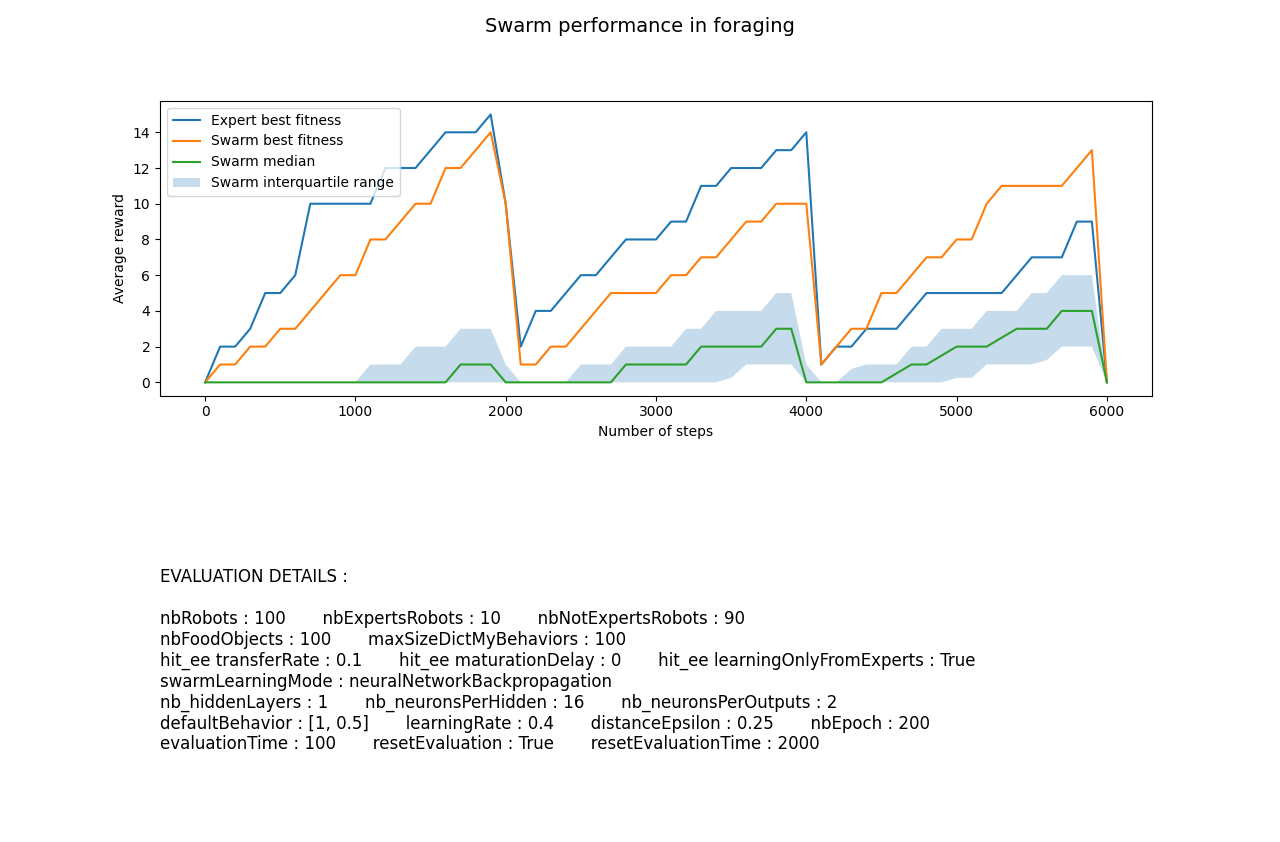
\includegraphics[scale=0.5]{bp6000_100.png}
    
    L'apprentissage par rétropropagation du gradient se révèle efficace et confère à chaque individu un mouvement continu qui n'imite pas parfaitement le comportement de l'expert mais assure la poursuite des mêmes objectifs. Cette proprièté permet parfois d'avoir des résultats meilleurs en termes de performances par rapport à ceux des experts. 
    Dans le graphique, on observe qu'à la troisième évaluation le meilleur individu non-expert de l'essaim obtient une meilleure performance par rapport à celle de l'expert observé. On remarque aussi la progressive amélioration de la performance des individus apprenants, ce qui entraîne une diminution des scores de l'expert de part la raréfaction des ressources.


    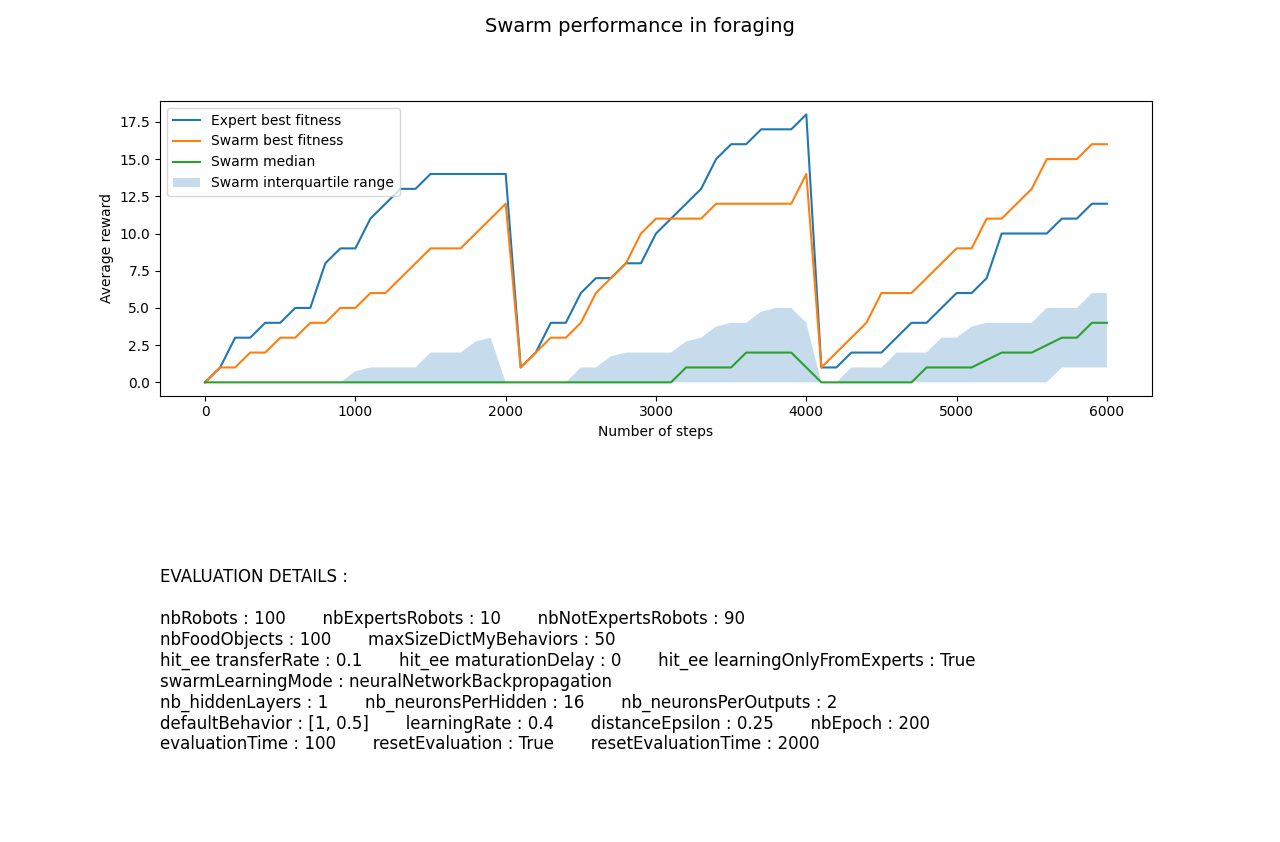
\includegraphics[scale=0.5]{bp6000_50.png}

    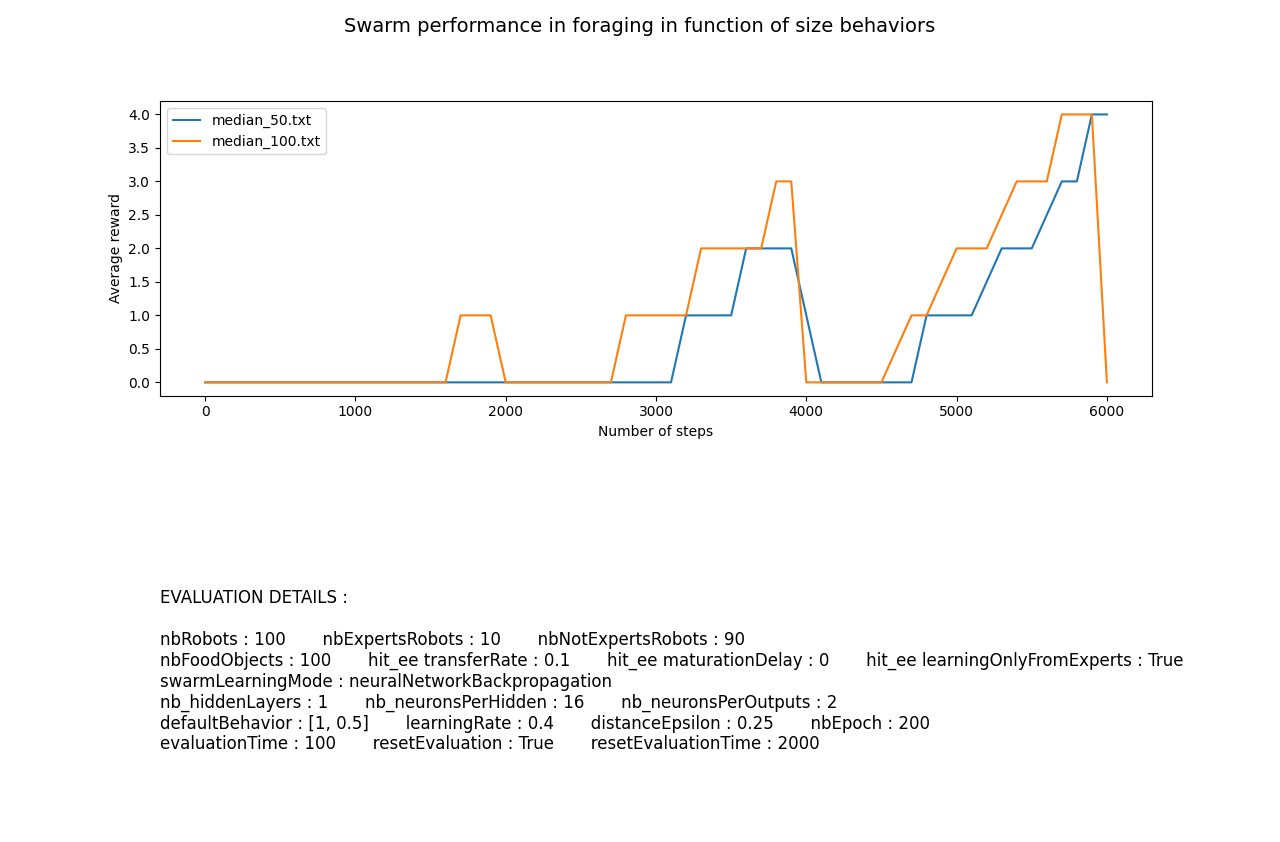
\includegraphics[scale=0.5]{sizeDB_50vs100_bp.png}

    La limitation de la base de données des individus focaux à 50 éléments (sur 100 traces totales possiblement pouvant être apprises des experts) réduit légèrement la capacité de l'essaim à apprendre de l'expert. 


    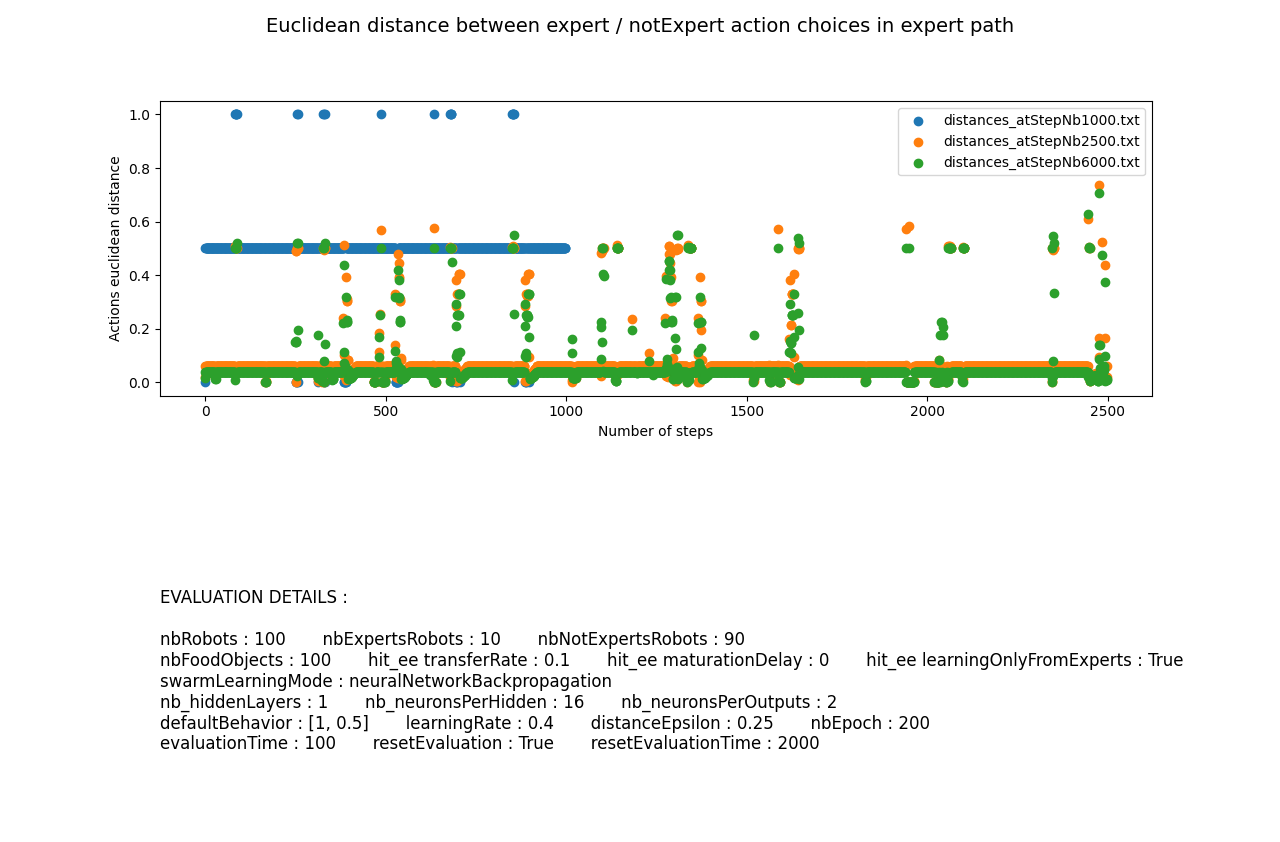
\includegraphics[scale=0.5]{distances_bp.png}

    Les choix effectués par le meilleur individu focal en termes d'actions s'améliorent au cours du temps. La bande verte réprésente une distance minimale entre l'action de l'individu focal et l'action de l'expert au moment $t = 6000$ step.
    Nous remarquons que le meilleur individu focal a déjà trouvé des poids efficaces pour le réseau de neurones au moment $t = 2500$ step.

    \subsection{Apprentissage par k Plus Proches Voisins}
    L'apprentissage par k Plus Proches Voisins permet d'observer une modification nette des comportements chez les individus focaux : les trajectoires changent rapidement suite à la phase d'entraînement, et ressemblent au comportement d'un individu expert. Cela est dû au fait que chaque action, sélectionnée par l'apprentissage de l'individu focal, correspond exactement à au moins une action de la base de données de l'expert, sans perte d'information.
    
    
    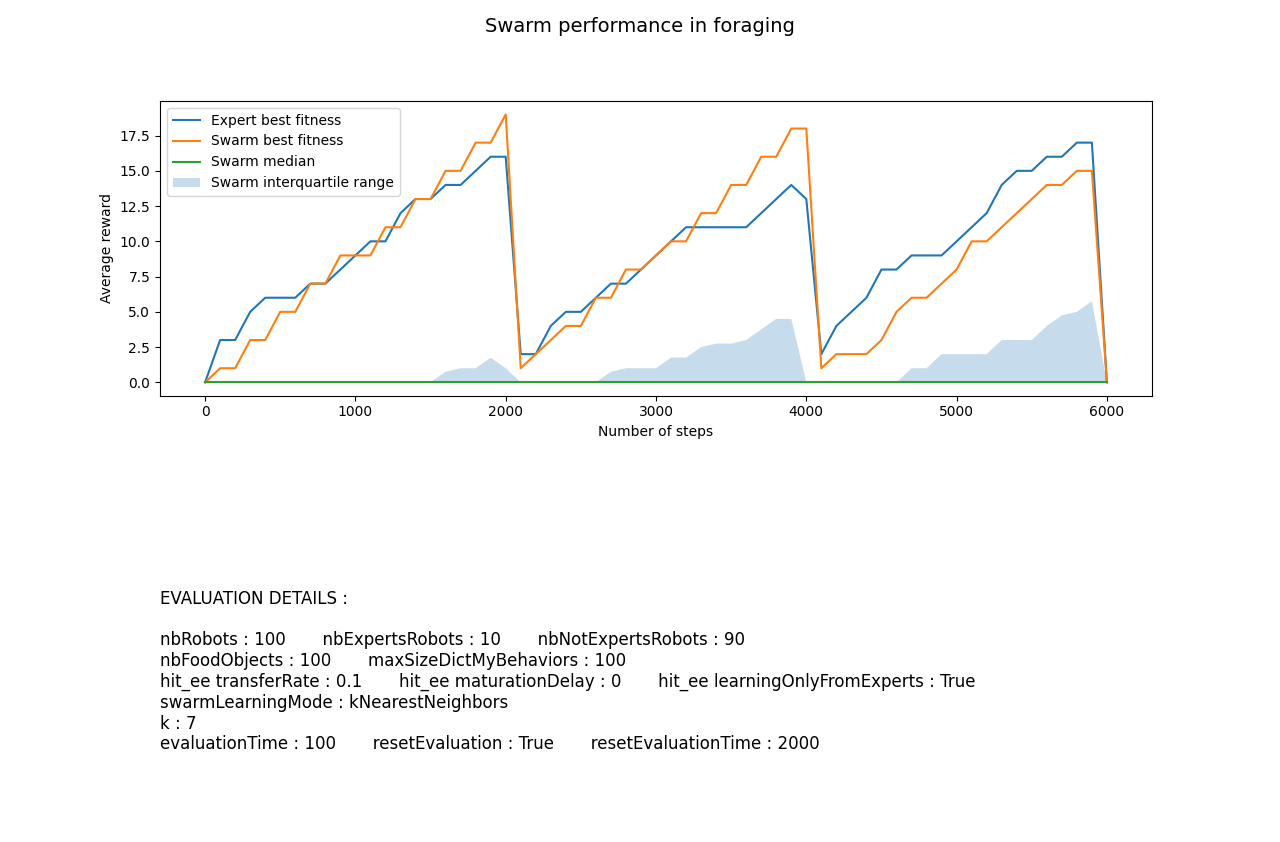
\includegraphics[scale=0.5]{knn6000_100.png}
    
    L'apprentissage par k Plus Proches Voisins est efficace et tend à imiter parfaitement le comportement de l'expert.
    Dans le graphique, nous pouvons voir que les performances du meilleur apprenant et de l'expert sont presque superposées. La connaissance générale du groupe évolue en fonction du temps mais progresse moins vite par rapport à l'apprentissage par rétropropagation du gradient.
    
    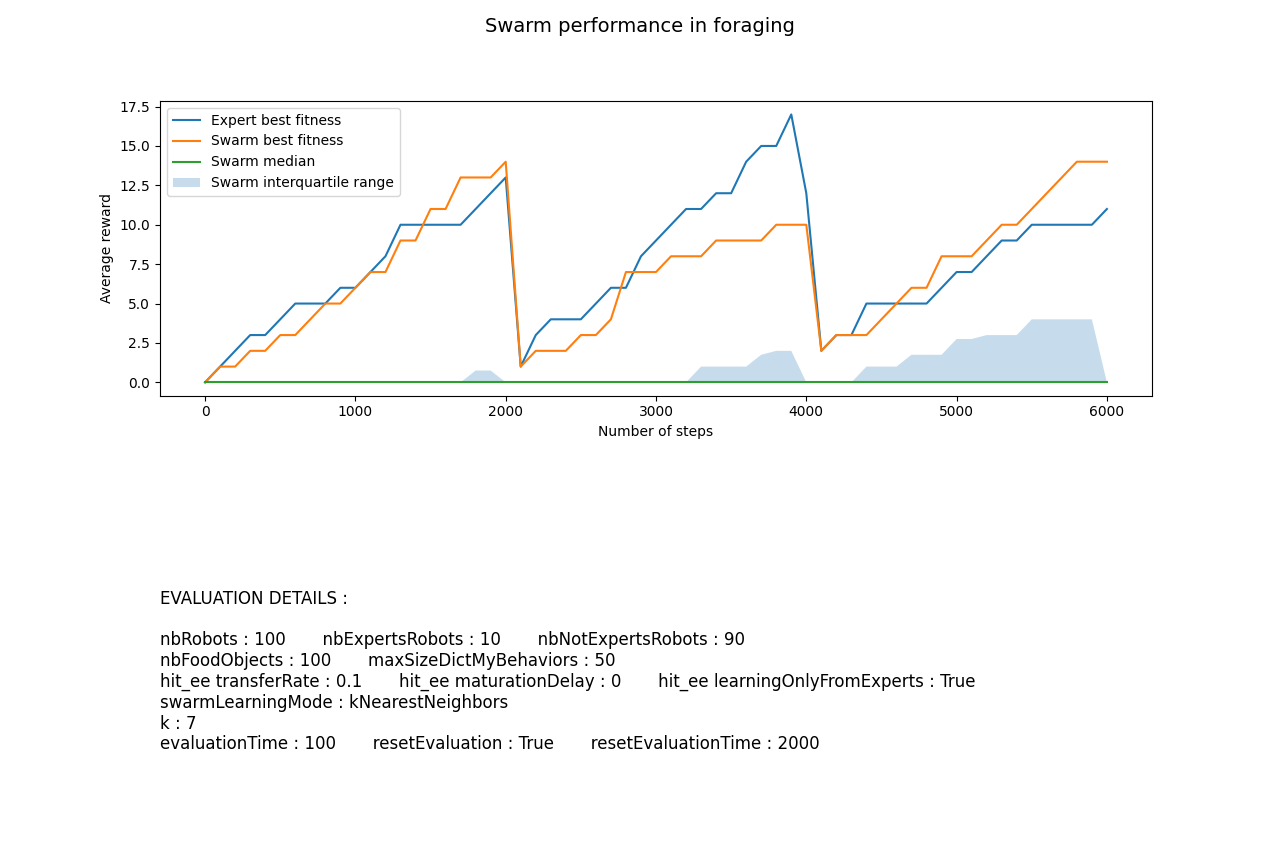
\includegraphics[scale=0.5]{knn6000_50.png}
    
    La limitation de la base de données des individus focaux à 50 éléments (sur 100 traces totales qui peuvent être apprises des experts) réduit la capacité de l'essaim à apprendre de l'expert. 
    
    
    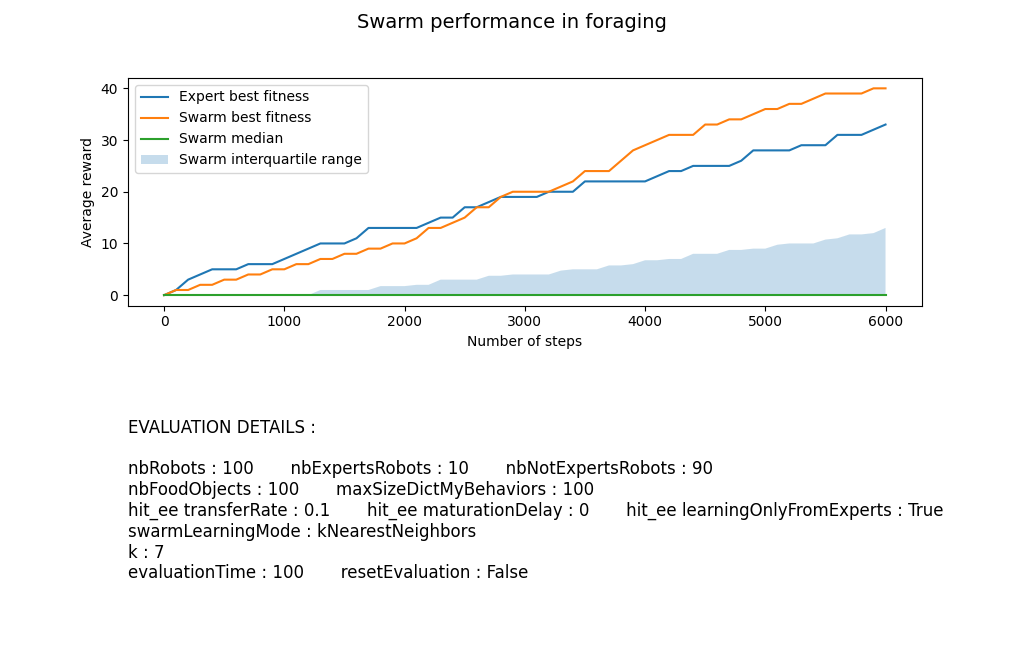
\includegraphics[scale=0.5]{knn6000_100_noReset.png}
        
    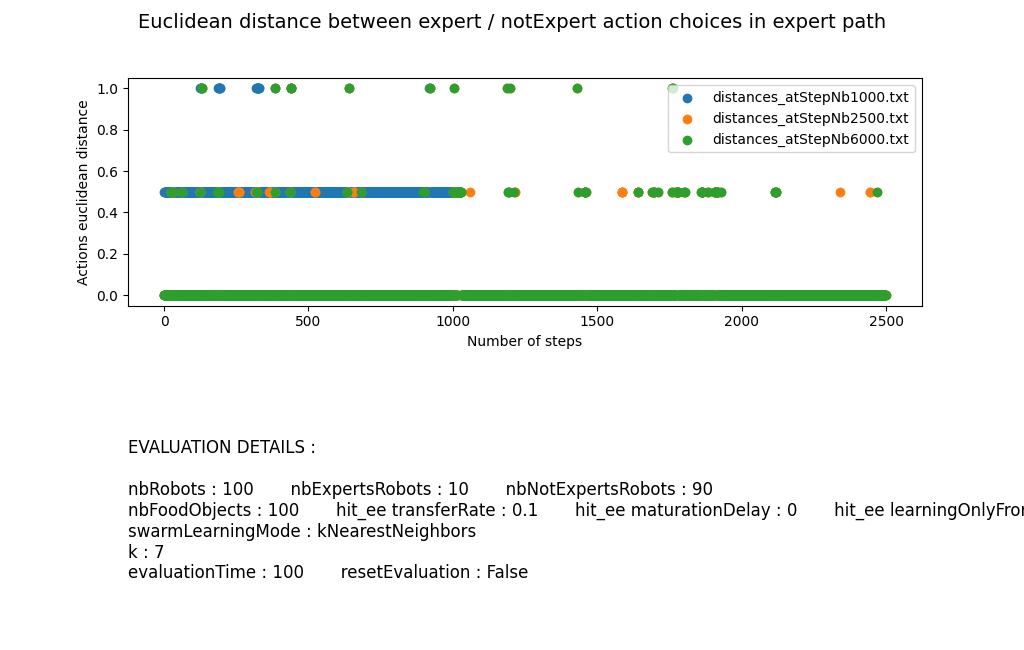
\includegraphics[scale=0.5]{distances_knn.png}
    
    Ce graphique des distances entre actions est obtenu à partir de l'expérimentation de 6000 steps sans réinitialisation des conditions initiales. Nous remarquons qu'en fin d'évaluation, l'essaim a un comportement beaucoup plus proche de celui de l'expert - en termes d'actions choisies - par rapport au début de l'évaluation.
    
    
	\section{Méthode par mimétisme}
	On décide ensuite de généraliser l'apprentissage en ajoutant de nouvelles contraintes : pour qu'un individu apprenne un comportement, ce dernier doit être observé. On change ainsi les informations transmises lors de la rencontre entre deux individus en un couple (observation, action) envoyé par l'expert.
	Pour simplifier, on ne considère pas la perte d'information due au changement de point de vue.
	\subsection{Apprentissage ad-hoc}
	Dans un premier temps, on se propose d'évaluer l'apprentissage par mimétisme en donnant aux apprenants une mémoire extensible et en déterminant le comportement des agents non-experts de la manière suivante :

\fbox{
	\begin{algorithm}[H]
		\KwInput{une observation $o$}\;
		\KwResult{l'action à effectuer $a$ }
  		On cherche l'observation $o'$ présente dans la mémoire telle que la distance $o$-$o'$ soit minimale\;
		L'observation $o'$ étant stockée avec une action $a'$ associée : $a$ $\leftarrow$ $a'$ \;
  		return $a$\;
	\end{algorithm}}
	
	La première remarque que l'on puisse faire sur cette méthode d'apprentissage est qu'en plus d'être coûteuse en mémoire, la simulation dure très longtemps. Ceci s'explique par le fait que les observations appartiennent à des segments continus compris entre 0 et 1 ce qui fait que la quasi totalité des comportements observés sont stockés et ensuite mesuré lors du calcul du plus proche voisin.
	
	De plus, lorsqu'un apprenant intègre un comportement, celui-ci est toujours dans le rayon de perception de l'expert, ce qui entraîne une perte de généralisation. Par exemple, les situations où un agent se retrouve en face d'un objet sans qu'aucun autre agent ne soit détecté par ses senseurs, ne peuvent être apprises.
	Pour palier à ce problème pour cette algorithme, on a fait le choix de ne transmettre que les informations des capteurs frontaux.
	Lorsque l'on ajoute l'apprentissage inter-apprenants, on observe rapidement un problème : un agent non-expert peut apprendre un mauvais comportement. Pour l'instant, l'on n'a aucun moyen de filtrer ou d'éliminer ces comportements sub-optimaux.
	
	\subsection{Apprentissage ad-hoc avec discrétisation des entrées}
	Afin d'adapter la méthode ad-hoc au domaine de la robotique en essaim, et donc de limiter la mémoire nécessaire, on a essayé de discrétiser les entrées. Une telle méthode a plusieurs avantages : elle réduit le domaine des observations $$nombre d'intervalles^{nombre de senseurs}*2^{nombre de senseurs de typage} $$ et permet de hasher ces dernières pour accéder plus efficacement aux comportements.
	Pour cette version, le comportement des apprenants suit les règles suivantes :
	
\fbox{
\begin{algorithm}[H]
	\KwInput{une observation $o$}\;
	\KwResult{l'action à effectuer $a$ }
	$o'$ $\leftarrow$ Discrétiser($o$)\;
	\If{o' est une clé du dictionnaire $mémoire$}								
	{\Return mémoire[$o'$]}
	\Return mouvement par défaut\;
\end{algorithm}}
	
	
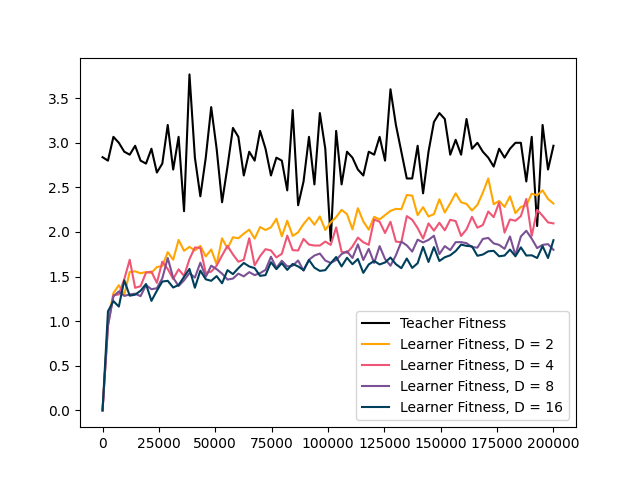
\includegraphics{averageComparisons}


	Par ces analyses, on remarque que lorsque le nombre d'intervalles de discrétisation augmente, la convergeance est de plus en plus lente. Ceci s'explique par un plus grand nombre de comportements à apprendre.
	 Cette supposition est confirmée par la quantité de mouvements appris en fonction du nombre d'intervalles de discrétisation.


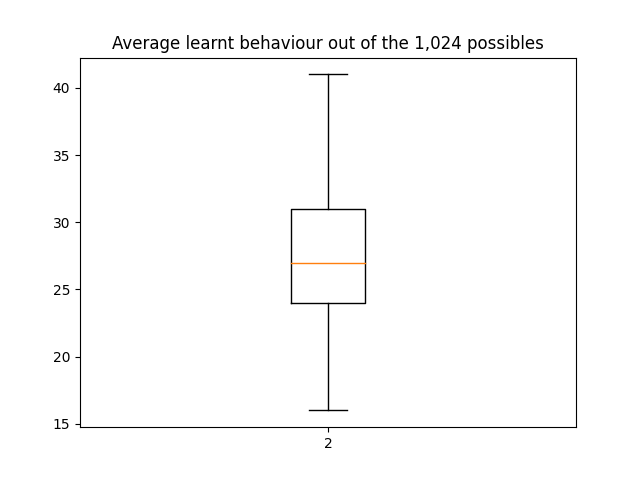
\includegraphics[scale = 0.5]{averageLearntBehaviourD2}
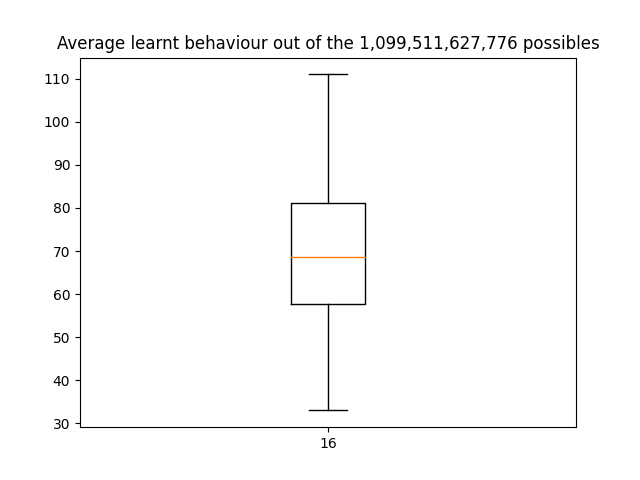
\includegraphics[scale = 0.5]{averageLearntBehaviourD16}
	
	En revanche, si le nombre d'intervalles est insuffisant, une partie du comportement de l'expert peut être perdue. Par exemple, si un expert adopte trois comportements différents en fonction de la valeur du senseur 1, une discrétisation en deux intervalles (respectivement [0,0.5], ]0.5,1]) ne permettrait pas l'apprentissage exact de ce comportement.
	
	Pour implémenter la propagation, il suffit de modifier la règle d'apprentissage de la manière suivante :
	
	%// Pseudocode
\fbox{
\begin{algorithm}[H]
	Lors de la réception d'un message $m$\;
	$o$,$a$ $\leftarrow$ $m$
	\If {$a\neq$ action par défaut}{$o'\leftarrow$discrétiser($o$)
	\If {$o'$ n'est pas une clé de du dictionnaire $mémoire$}{$mémoire$[$o'$] $\leftarrow a$}}
\end{algorithm}}
	
	
	\textbf{N.B.} Pour les tests, on a fait le choix de définir le mouvement par défaut comme (0.5, 0.05), c'est-à-dire de continuer tout droit, mais avec un léger déplacement vers la droite pour éviter aux agents de se coincer.

\begin{center}
	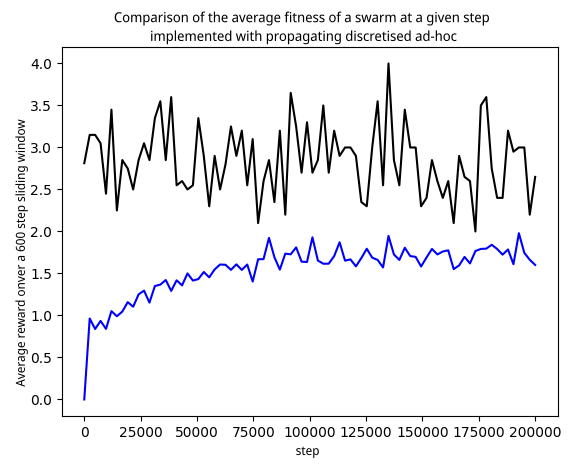
\includegraphics{D2Propag}
\end{center}	
A première vue, cette expérience semble donner des résultats moins bons que sans propagation, mais elle n'est pas représentative, car nous avons dû limiter le nombre de répétitions de l'expérience par manque de temps. Il faudrait donc refaire cette expérience en la comparant à sa version sans propagation, et ce sur un nombre représentatif d'expériences.
	
	
	\subsection{Apprentissage ad-hoc avec plus proche voisin}
	Une autre option envisagée pour réduire la demande en mémoire de notre algorithme est de toujours exécuter l'action de la mémoire dont l'observation est la plus proche de l'observation actuelle.
	De plus, afin de limiter le nombre de points insérés dans la mémoire, on a implémenté l'algorithme suivant :

\fbox{
\begin{algorithm}[H]
	\SetAlgoLined
	Lors de la réception d'un message $m$\;
	$o$,$a$, $w$ $\leftarrow$ $m$
	On cherche le couple ($o'$, $a'$) tel que la distance $o-o'$ soit minimale\;
	\If{$a\neq a'$}{On ajoute le tuple ($o$, $a$, 1) à la mémoire}{On modifie $o$ de la manière suivante\;
	$o'\leftarrow$ ( $ \frac{o'* w + o}{w+1}$}
\end{algorithm}}
	
Les principales différences observées lors de ces tests sont dues au choix de l'heuristique de calcul de distance. En effet, une heuristique de simple calcul de distance euclidienne a comme défaut de ne pas prendre en compte le type des objets rencontrés (ceux ci étant encodés sous forme de booléens 0,1). Une solution est d'utiliser une heuristique maximin, mais les résultats restent insuffisants.
Au final, nous avons fait le choix de projeter les distances aux obstacles sur différents hyperplans correspondants aux différentes permutations du type d'objet rencontré, puis effectué le calcul de la distance euclidienne.

L'inconvénient majeur de cette méthode est la difficulté à l'adapter à la propagation entre apprenants. Simplement permettre cette dernière provoquerait l'apprentissage de "mauvais" comportements qui limiteraient à long terme la convergence de l'efficacité de la population.

Une solution envisagée à été de calculer pour chaque observation faite la vraisemblance du mouvement associé à cette observation. Mais cette méthode, très calculatoire, demandait une grande mémoire pour avoir une base de comparaison.
	
	\subsection{Apprentissage sur un réseau de neurones par Backpropagation}
	Pour remédier aux différents problèmes remarqués dans les méthodes ad-hoc, on a essayé d'appliquer l'apprentissage par mimétisme sur un réseau neuronal. Ainsi, la présence d'un agent sur un senseur donné devrait disparaître lors de la généralisation.
	Un problème s'est néanmoins présenté : certaines observations sont beaucoup plus représentées que d'autres.
	
\begin{center}
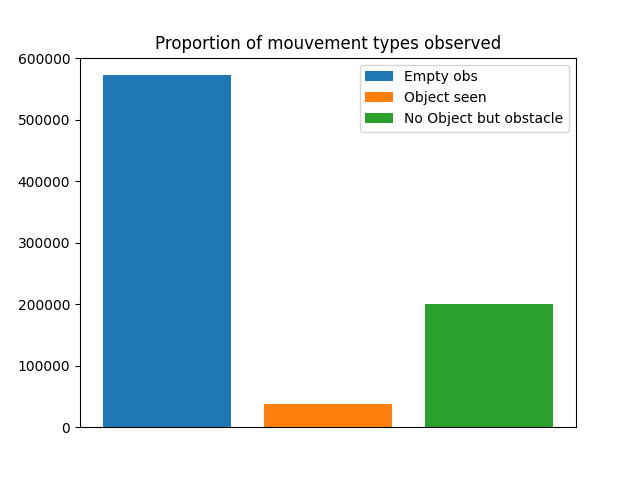
\includegraphics[scale = 0.5]{Proportions}
\end{center}	

	Pour palier à cela, on a donc renforcé l'apprentissage en pondérant la rétropropagation lors de l'apprentissage en fonction de la distance à l'objectif.

\begin{center}
	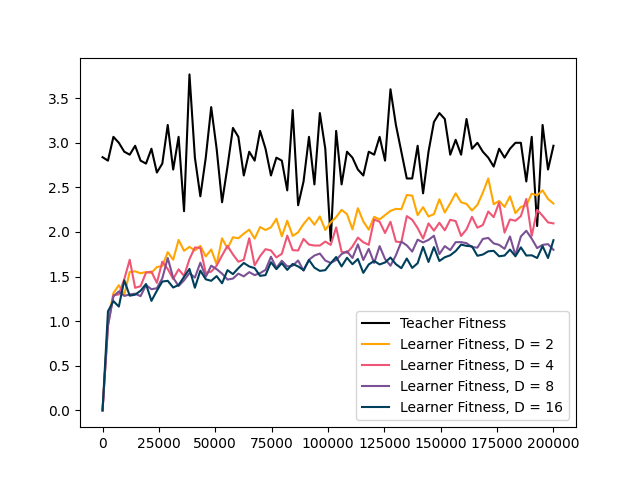
\includegraphics{averageComparisons}
\end{center}	
	
Cette méthode est, comme attendu, plus lente que la version ad-hoc. En revanche elle semble suivre une croissance continue. Il serait envisageable de poursuivre l'expérience jusqu'à la stabilisation de la population.
	
\begin{center}
	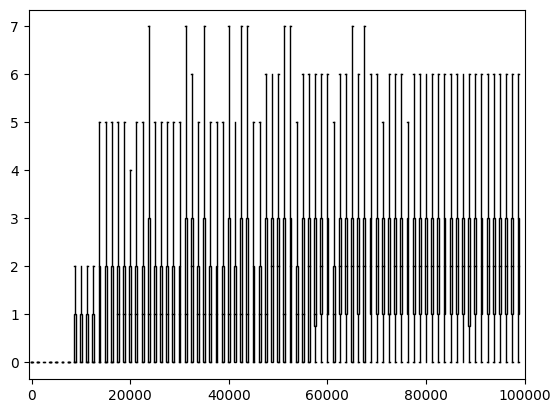
\includegraphics{learner_boxplot}
\end{center}	

	En permettant en plus à l'apprentissage d'avoir lieu entre apprenants, on observe que la moyenne ne semble pas s'améliorer plus vite que dans l'expérience précédente. Néanmoins, l'ensemble de la population évolue de manière plus homogène.


\chapter{Conclusion}

A première vue, l'apprentissage par comportement au sein d'un essaim de robots semble être une méthode prometteuse pour l'apprentissage à moindre coût.

Néanmoins, avant de pouvoir vraiment la comparer à d'autres méthodes existantes et la tester dans le monde réel, il faudrait déjà la tester avec la perte de connaissances qu'induit un changement de perspective.
\begin{center}
	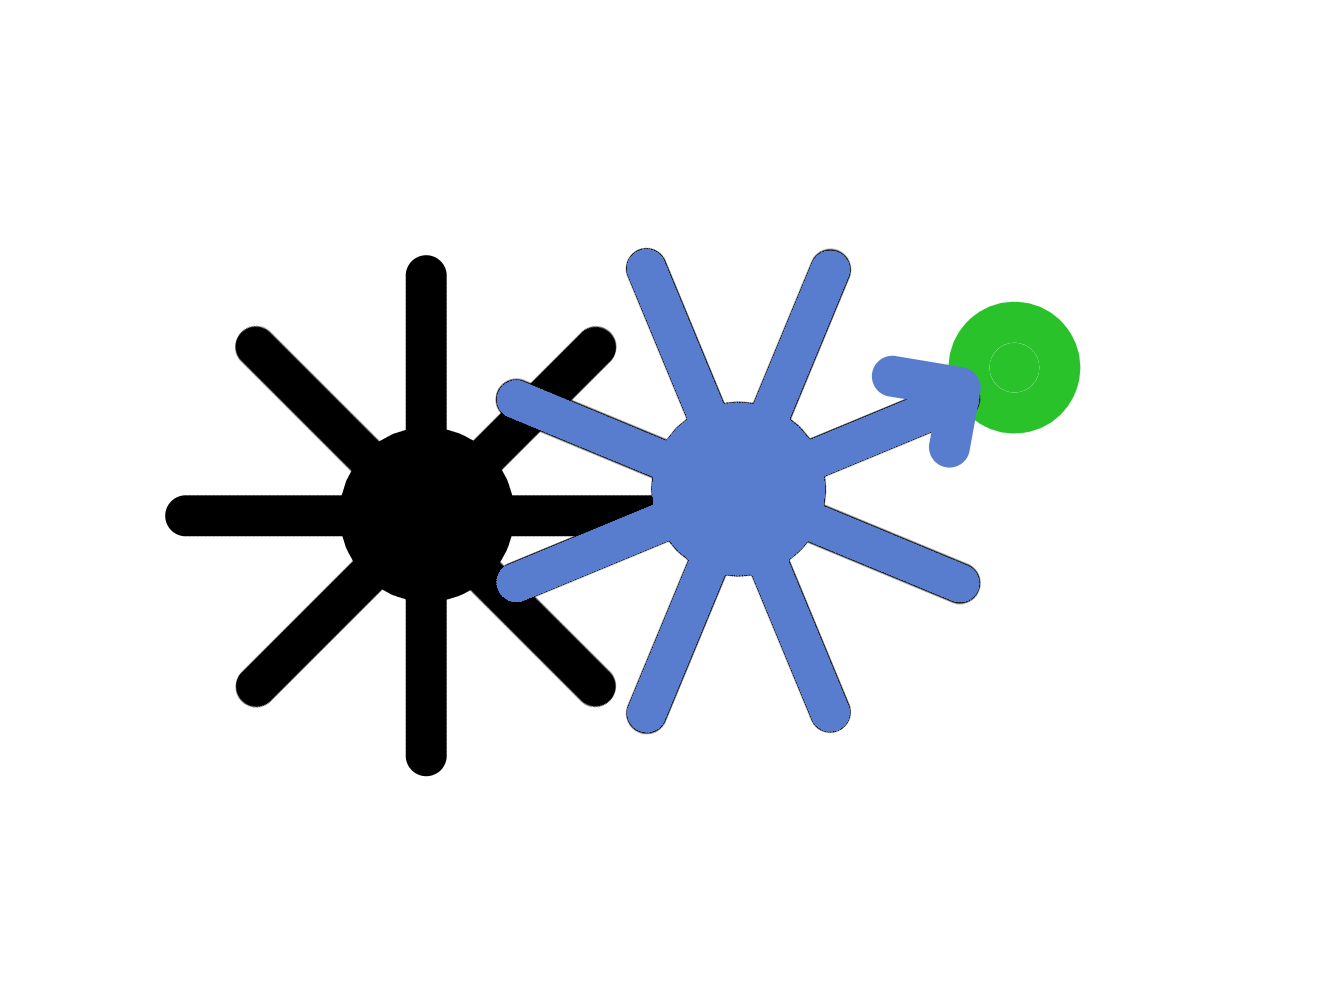
\includegraphics[scale = 0.5]{scheme.png}
\end{center}
\textit{Dans l'exemple ci-dessus, l'apprenant(en noir), ne voit pas l'objet(en vert) vers lequel se dirige l'expert(en bleu), pour lui l'expert ne détecte aucun objet à part l'apprenant.}

De plus, certaines de nos expériences n'ont pu avoir de résultats représentatifs par manque de temps. Ainsi, pour la poursuite de notre projet, nous devrions optimiser les différents codes pour permettre des expériences plus représentatives, pour ensuite pouvoir comparer nos résultats avec les algorithmes "state of the art"

    \appendix
    \chapter{Bibliographie}
\begin{itemize}
	\item{Nicolas Bredeche and Nicolas Fontbonne. 2022. Social learning in swarm robotics. Philos. Trans. R. Soc. B Biol. Sci. 377, 1843 (January 2022), 20200309. DOI:https://doi.org/10.1098/rstb.2020.0309}
 \end{itemize}
    %\printbibliography


    \chapter{Cahier des charges}
    \begin{figure}[H]
		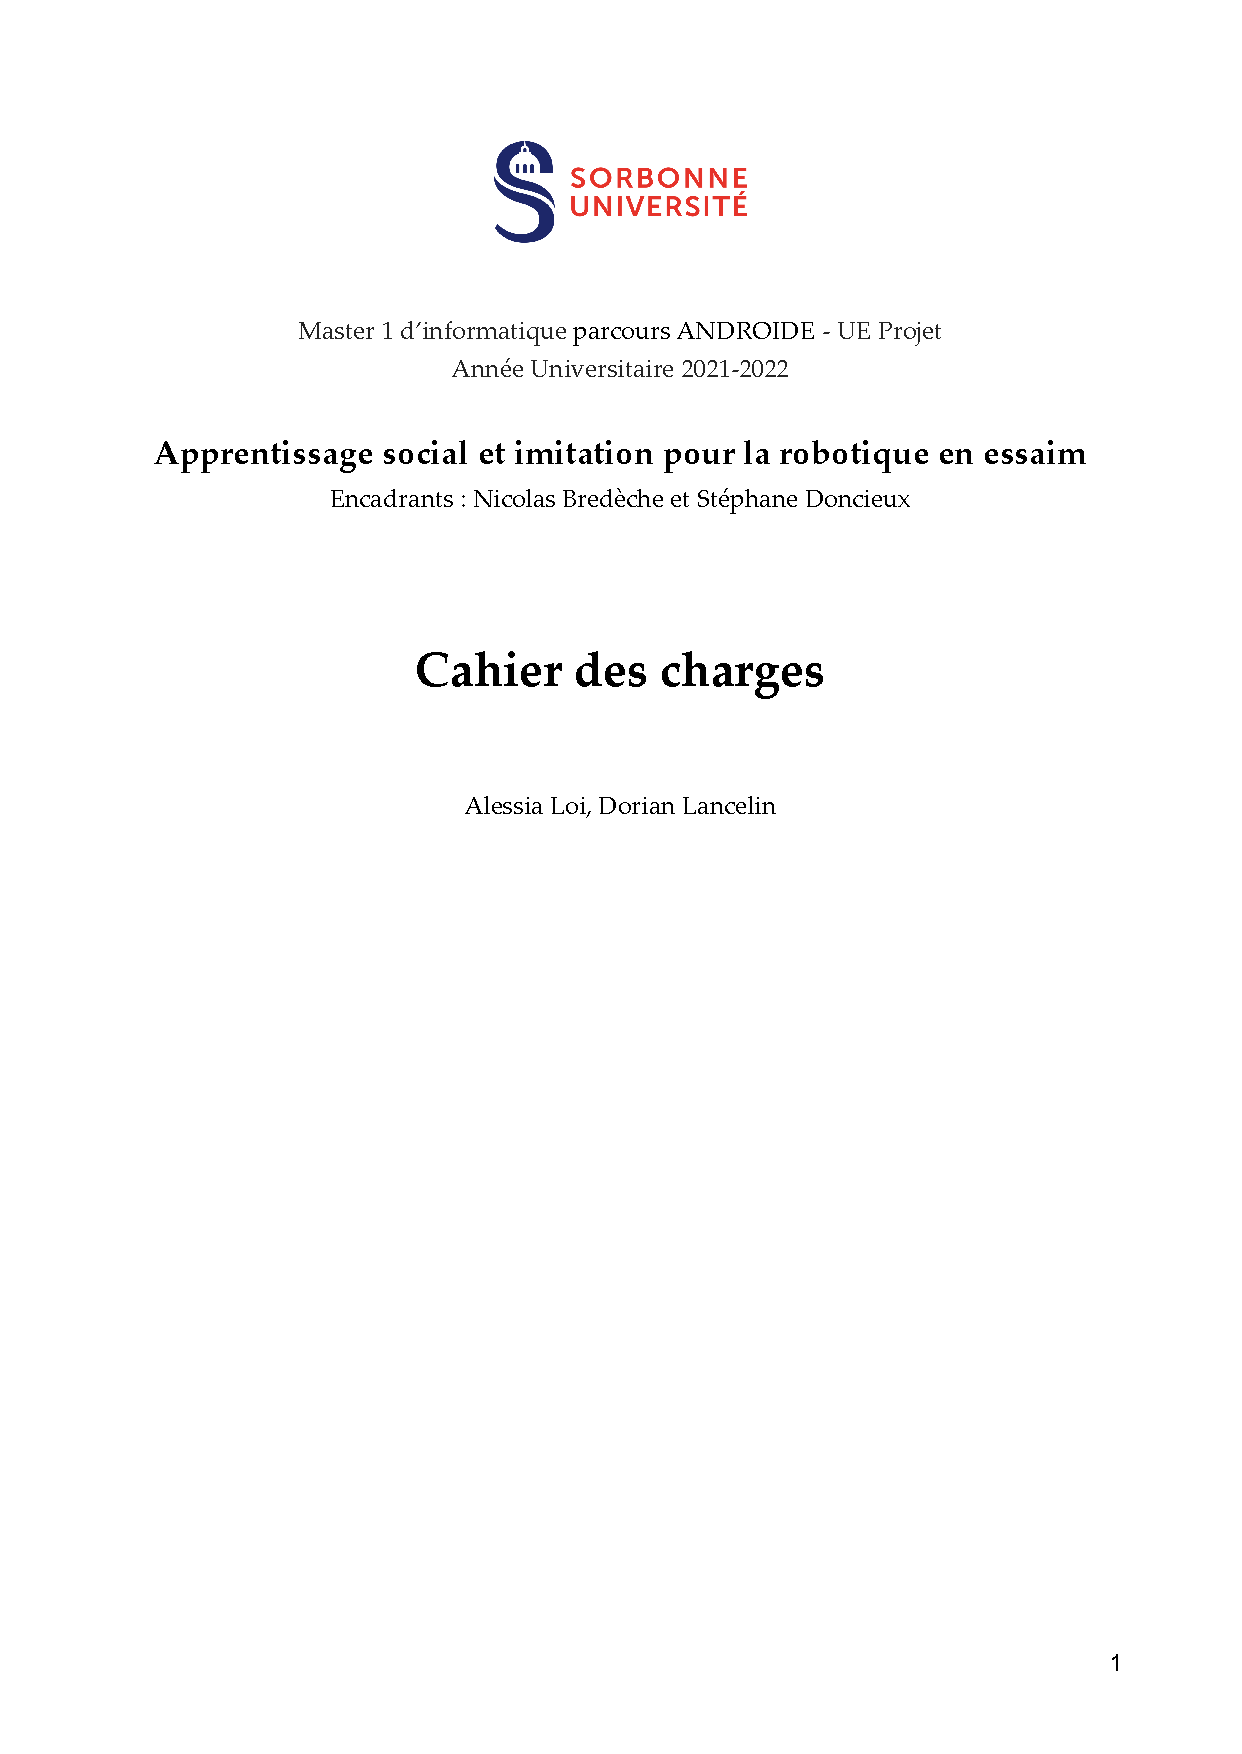
\includepdf[scale = 0.9,nup=2x2, pages=1-4]{CDC.pdf}
    \end{figure}
    \chapter{Manuel utilisateur}
     
    \subsection{Méthode par transmission de comportements}
    
    \begin{itemize}
        \item Se positionner sur le répertoire \textit{ASIRE\_project}
        
        \item Dans le fichier \textit{part2\_main\_diffusion.py}, en début de page, fixer les paramètres à utiliser :
        
        \begin{itemize}
        \item section \textbf{\textit{configuration file parameters}}. Fixer le nombre de individus experts \textit{nbExpertsRobots}, le nombre d'individus focaux \textit{nbNotExpertsRobots} et le nombre d'objets \textit{nbFoodObjects} pour l'expérience. Remarque : il ne faut pas modifier le fichier de configuration qui se trouve dans le répertoie \textit{config}.
        \item section \textbf{\textit{learning mode configuration}}. Choisir la mèthode d'apprentissage pour l'expérience courante : commenter la ligne de la mèthode à ne pas utiliser.
      \item section \textbf{\textit{parameters}}. Fixer le nombre total de steps \textit{nbSteps} de l'expérience et la taille de la base de données des individus \textit{maxSizeDictMyBehaviors}. Affecter \textit{True} à la variable \textit{learningOnlyFromExperts} pour limiter la possibilité de diffuser ses traces comportamentales aux seuls individus experts; affecter \textit{False} pour permettre à tous les individu de diffuser ses propres traces comportamentales.
            \item section \textbf{\textit{debug and plot parameters}}. Il est possible de visualiser les détails d'execution des algorithmes en affectant la valeur \textit{True} aux différentes variables \textit{debug\_*}.
            
        \end{itemize}
        
        Remarque : le fichier \textit{part2\_bestParameters.txt} conserve une copie des meilleurs paramètres testés lors des expériences.
        
        \item Exécuter le fichier \textit{part2\_main\_diffusion.py}.
    
    \end{itemize}
    
    \subsection{Méthode par mimétisme}
Comment recréer les expériences citées :

Installer \href{https://github.com/nekonaute/roborobo4}{Roborobo} et lancer une instance d'Anaconda.

Se déplacer dans le dossier $mimetic_Learning$ :

Choisir les paramètres dans le fichier Cons.py :
\begin{itemize}
\item\textbf{Global}
	\begin{itemize}
		\item{VERBOSE = True / False}
		\item{$DATA\_SAVE$ = True / False}
		\item{$SAVE\_FILE$ = "filepath"}
		\item{$OVERWRITE\_FILE$ = True / False}
	\end{itemize}
\item\textbf{ExtendedAgents}
\textit{Options pour l'apprentissage par réseau de neurones}
	\begin{itemize}
		\item{$NB\_HIDDENS$ = int}
		\item{$EVALUATION\_TIME$ = 600				\textit{Taille de la sliding window}}
		\item{$MEMORY\_RANGE$ = 20}
		\item{$LEARNING\_STEPS$ = 30		\textit{Nombre de répétitions de la phase d'apprentissage}}
		\item{$LEARNING\_RATE$ = 0.8}
		\item{$MUTATION\_RATE$ = 0.}
	\end{itemize}
\item{\textbf{Foraging Task}}
	\begin{itemize}
		\item{$LEARNING\_ALGORITHM$ = "adhoc"        \textit{"adhoc" or "neural"}}
		\item{$NB_ITEMS$ = 100						\textit{Nombre d'objets instanciés}}
		\item{$REGROWTH\_TIME$ = 10	\textit{Durée avant réapparition des objets}}
		\item{$CHANGE\_POSITION$ = True				\textit{Si les objets réapparaissent à d'autres endroits}}
		\item{$NB\_ITER$ = 200000					\textit{Durée de l'expérimentation}}
	\end{itemize}

\item{\textbf{NeuralLearner}}
	\begin{itemize}
		\item{$PROPAGATION$ = False					\textit{Apprentissage apprenant - apprenant}}
		\item{$DECAY\_FUNCTION$ = constantLearningRate	\textit{Choix de la fonction de réduction du taux} d'apprentissage}
		\item{$DECAY\_RATIO$ = 0.01}
	\end{itemize}

\item{\textbf{MemoryAgents}}
	\begin{itemize}
		\item{$EXPERT\_SPEED$ = 1}
		\item{$LEARNING\_GAP$ = 60}										
		\item{$MEMORY\_SIZE$ = 100					\textit{Nombre de messages stockés simultanément}}
		\item{$NB\_LEARNER$ = 90						\textit{Nombre de robots apprenants}}
		\item{$DISCRETISE\_RATIO$ = 2                \textit{Si -1 : plus proche voisin}}
		\item{$LEARNT\_BEHAVIOUR\_PROPAGATION$ = False \textit{Apprentissage apprenant - apprenant}}
	\end{itemize}
\end{itemize}
Exécuter le runner:
python $Foraging\_Task$
\end{document}
